\section{Evaluations} \label{Evaluations}

\subsection{Base Core Parameters}

The two attacks were replicated on the BOOM core with the parameters given
in Table \ref{tab:boom-core-params}. Note that our configuration employs 4 MSHRs and thus contains a 4-entry SpecBuf.
We have used the "simple" version of the PNR for the results (Section \ref{Point of No Return}), as the fast version has not yet provided a measurable performance increase.
All attacks were measured using FireSim, an open-source cycle-accurate, FPGA-accelerated scale-out computer system simulation platform \cite{b12}.

\begin{table}
\centering \caption{BOOM Core Parameters} \label{tab:boom-core-params}
\begin{tabular}{@{} *2l @{}} \toprule
    Parameter                    & Value \\ \midrule
    Fetch Width                  & 2 \\
    Decode Width                 & 2 \\
    Issue Width                  & 4 \\
    PRF Size                     & 100 \\
    ROB Size                     & 100 \\ \midrule
    L1 Sets                      & 64 \\
    L1 Ways                      & 8 \\
    L1 Linesize                  & 64 bytes \\
    MSHR File Entries            & 4 \\ \midrule
    BTB Sets                     & 512 \\
    BTB Banks                    & 2 \\
    BTB Ways                     & 4 \\ \midrule
    GShare History Bits          & 23 \\
    GShare Counter Table Entries & 4096 \\ \bottomrule
\end{tabular}
\end{table}

\begin{figure}
    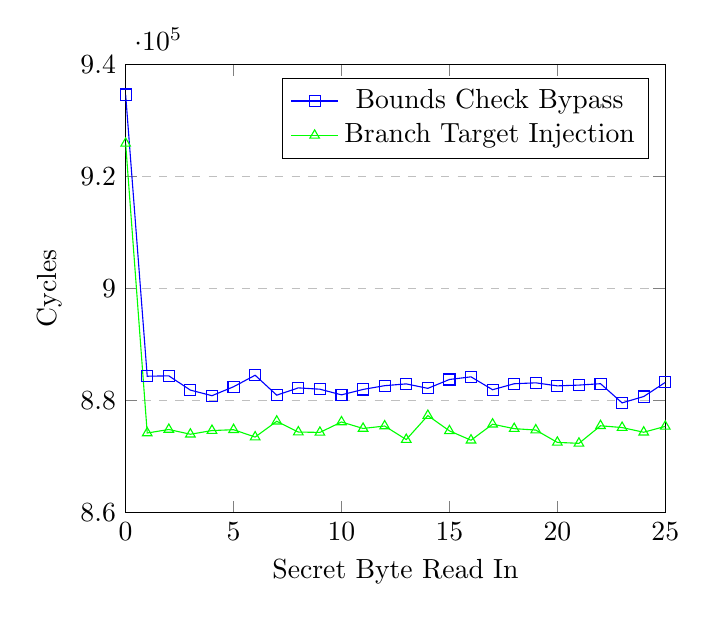
\begin{tikzpicture}
        \begin{axis}[
            ylabel={Cycles},
            xlabel={Secret Byte Read In},
            xmin=0, xmax=25,
            ymin=860000, ymax=940000,
            legend pos=north east,
            ymajorgrids=true,
            grid style=dashed
        ]
            \addplot[
                color=blue,
                mark=square,
            ]
            coordinates {
                (0 ,934580)
                (1 ,884322)
                (2 ,884387)
                (3 ,881845)
                (4 ,880847)
                (5 ,882446)
                (6 ,884498)
                (7 ,880939)
                (8 ,882241)
                (9 ,882006)
                (10,880994)
                (11,881965)
                (12,882634)
                (13,882954)
                (14,882156)
                (15,883738)
                (16,884212)
                (17,881912)
                (18,882980)
                (19,883142)
                (20,882600)
                (21,882739)
                (22,882989)
                (23,879563)
                (24,880698)
                (25,883218)
            };
                    
            \addplot[
                color=green,
                mark=triangle,
            ]
            coordinates {
                (0 ,925862)
                (1 ,874188)
                (2 ,874815)
                (3 ,873968)
                (4 ,874626)
                (5 ,874778)
                (6 ,873466)
                (7 ,876281)
                (8 ,874361)
                (9 ,874297)
                (10,876153)
                (11,875000)
                (12,875435)
                (13,873015)
                (14,877303)
                (15,874572)
                (16,872902)
                (17,875761)
                (18,874966)
                (19,874715)
                (20,872514)
                (21,872346)
                (22,875481)
                (23,875161)
                (24,874325)
                (25,875371)
            };
            \legend{Bounds Check Bypass,Branch Target Injection}
        \end{axis}
    \end{tikzpicture}
    \caption{Speed of Replicated Attacks}
    \label{fig:speed-attacks}
\end{figure}

\subsection{Replicating Speculative Attacks Results}

Overall, the attacks chosen were replicated successfully on the BOOM microarchitecture. A printout
demonstrating leakage of secret information with the Bounds Check Bypass attack
is shown in Code \ref{code:spec-attack-printout}. Initial results of the replications
are promising with around 3.6KB/s for both attacks. Table \ref{tab:spec-attack-results}
shows the results of the two attacks while Figure \ref{fig:speed-attacks} shows the cycles per secret byte read out.
These measurements take into account the clearing
of the tally array before each run, the multiple rounds of training for the BPU,
the single attack run on the victim, and the time to measure out the secret from the attacker array.
The cycle times are close to each other because the code shares a similar structure. The main
differences are around the setup of the {\tt fdiv} manipulation
and the extra arithmetic in the Branch Target Injection attack where you have to calculate
both the index and the address for accessing the function and passing the input. 

\begin{lstlisting}[style=column-code, label={code:spec-attack-printout}, caption=Printout of Bounds Check Bypass Attack]
want(#) =?= 1.(#) 2.( C)
want(T) =?= 1.(T) 2.(^A)
want(h) =?= 1.(h) 2.(i)
want(i) =?= 1.(i) 2.(>)
want(s) =?= 1.(s) 2.(^D)
want(I) =?= 1.(I) 2.(^D)
want(s) =?= 1.(s) 2.( ^L)
want(T) =?= 1.(T) 2.( )
want(h) =?= 1.(h) 2.(^F)
want(e) =?= 1.(e) 2.()
want(B) =?= 1.(B) 2.(<9f>)
want(a) =?= 1.(a) 2.(^B)
want(b) =?= 1.(b) 2.(^A)
want(y) =?= 1.(y) 2.()
want(B) =?= 1.(B) 2.( )
want(o) =?= 1.(o) 2.(^H)
want(o) =?= 1.(o) 2.(4)
want(m) =?= 1.(m) 2.(k)
want(e) =?= 1.(e) 2.(^C)
want(r) =?= 1.(r) 2.(^A)
want(T) =?= 1.(T) 2.(^C)
want(e) =?= 1.(e) 2.(^O)
want(s) =?= 1.(s) 2.(^D)
want(t) =?= 1.(t) 2.(^A)
\end{lstlisting}


\begin{table}
\centering
\caption{Attack Parameters}
\label{tab:attack-params}
\begin{tabular}{@{} *2l @{}} \toprule
    Parameter                    & Value \\ \midrule
    Cache Hit Threshold          & 50 cycles \\
    Amount of runs on same byte  & 10 rounds \\
    Training rounds for BPU      & 6 training rounds \\
    Cache flush hits on same set & 4 * L1\_WAYS \\
    GShare Counter Table Entries & 4096 \\ \bottomrule
\end{tabular}
\end{table} 

\begin{table}
\centering
\caption{Speculative Attack Results}
\label{tab:spec-attack-results}
\begin{tabular}{@{} *4l @{}} \toprule
    &                        & \multicolumn{2}{l}{Bytes per Second} \\
    Attack                  & Cycles for Secret Byte &           100 MHz &   3.2 GHz \\ \midrule
    Bounds Check Bypass     &                ~884485 &          ~113 B/s & ~3618 B/s \\
    Branch Target Injection &                ~876602 &          ~114 B/s & ~3650 B/s \\ \bottomrule
\end{tabular}
\end{table}

\subsection{SpecBuf Results} \label{SpecBuf Results}

We evaluated our SpecBuf implementation using three small microbenchmarks, Dhrystone and the 
replicated attacks. The microbenchmarks created stress the MSHR blocking and eviction conditions
that slow down the machine while Dhrystone was chosen as an initial general test. The SpecBuf shows an expected small decrease
in performance in the microbenchmark tests while Dhrystone shows a small improvement all while providing
a defense against the replicated attacks demonstrated. A table of results is shown at Table \ref{tab:spec-buf-results}.

\subsubsection{Microbenchmark Explanations and Results}

The first microbenchmark named "Non-speculative load misses to same sets" was used to test how efficient non-speculative loads
were when the MSHR was unable to allocated entries for each new load. This microbenchmark is a series of loads that had different
tags but the same index, thus in BOOM's MSHR, only one entry would be able to be allocated at a time. When using the SpecBuf, the 
behavior is similar. The main difference is that on each load, the data from cache hierarchy must first fill the MSHR buffer
before the cache. This causes a small performance decrease for each load. Since our benchmark has 16 loads, this results in a performance decrease of around
{\tt 16 loads * (CACHE\_LINE\_SZ / DATABUS\_WIDTH)} or {\tt 16 * (64B / 8B) = 128 cycles}.

The second microbenchmark named "Non-speculative load misses to different sets" is similar to the first except that each subsequent
load is accessing a different set in the cache. In the normal version of BOOM, the MSHRs would fill up completely but then stall 
when full until a prior MSHR entry would be freed (when a previous load is completed). When using the SpecBuf, there is a
higher performance penalty because the data must fill the MSHR buffer with the cache data before filling the cache. Thus, there 
is a extra overhead of around 8 cycles for every 4 loads since the MSHR's are allocated waves of 4 and the fill latency to the MSHR
buffer is {\tt CACHE\_LINE\_SZ / DATABUS\_WIDTH} or {\tt 64B / 8B = 8 cycles}.

The final microbenchmark named "MSHR evicted speculative load miss" is used to test the impact when a load has to be evicted from an 
MSHR due to a potential deadlock condition. For instance, consider two loads which miss to different addresses that map to the same cache index, keeping in mind the limitation discussed in Section \ref{Fully Associative MSHR File}. In the normal version of BOOM, if one of these loads is speculatively issued to an 
MSHR before a critical load that resolves the speculation, the speculative load will complete and
write its data to the cache. This will release the MSHR entry it occupied and allow the critical load to complete, resolving the speculation. 
However, with SpecBuf enabled, the speculative load will fill the data in the MSHR buffer, bypass the data to the microarchitectural register, 
then wait for speculation to finish to determine if the data will enter the cache. If the critical load that needs the MSHR is issued after the speculative load,
then the speculative load is evicted from the MSHR file. If the 
flow proved to be speculated correctly, then any following loads to the same cache line would miss, causing a performance decrease.
This microbenchmark shows the increased latency of a load to the evicted cacheline following this scenario.
Note that a similar scenario can arise when the MSHR file is filled by many speculative loads, in which case one of the speculative loads would be randomly selected for eviction.

\subsubsection{Dhrystone Results}
Enabling the SpecBuf granted a 2\% increase in Dhrystone performance, seen below in Table \ref{tab:spec-buf-results}. There are several factors which may contribute to this small performance gain. The SpecBuf delays the eviction of old cachelines until the refill is known to commit, allowing hits on the old cacheline in the intervening cycles. Additionally, the SpecBuf decreases the latency of missed loads: this is because refill requests can be sent to the bus earlier, and the retured data can be forwarded out of the buffer as soon as it is available, rather than waiting for the update of cache metadata.

\begin{table}
\centering
\caption{SpecBuf Results}
\label{tab:spec-buf-results}
\begin{tabular}{@{} *4l @{}} \toprule
    & \multicolumn{2}{l}{Version of BOOM} & \\
    Benchmark                           & Normal & SpecBuf & \% Diff.\\ \midrule
    Non-spec. LD misses   & 540 cycles & 640 cycles & -19\%    \\
    to same sets            &            &            & \\ \midrule
    Non-spec. LD misses   & 264 cycles & 297 cycles & -11\%    \\ 
    to diff. sets           &            &            & \\ \midrule
    MSHR evicted spec. & 48 cycles & 67 cycles & -40\%    \\
    LD miss                &            &            & \\ \midrule
    Dhrystone                           & 2176 Dhrystones/s & 2216 Dhrystones/s & +2\%\\ \bottomrule
\end{tabular}
\end{table}

\subsubsection{Synthesis Results} \label{Synthesis Results}
Trial synthesis of BOOM with our 4-entry SpecBuf in a 45nm technology resulted in a 2.5\% increase in area and a 0.36\% decrease in clock frequency using HAMMER, a framework to
abstract synthesis and place-and-route \cite{hammer}.


